\begin{figure*}[t]
\centering
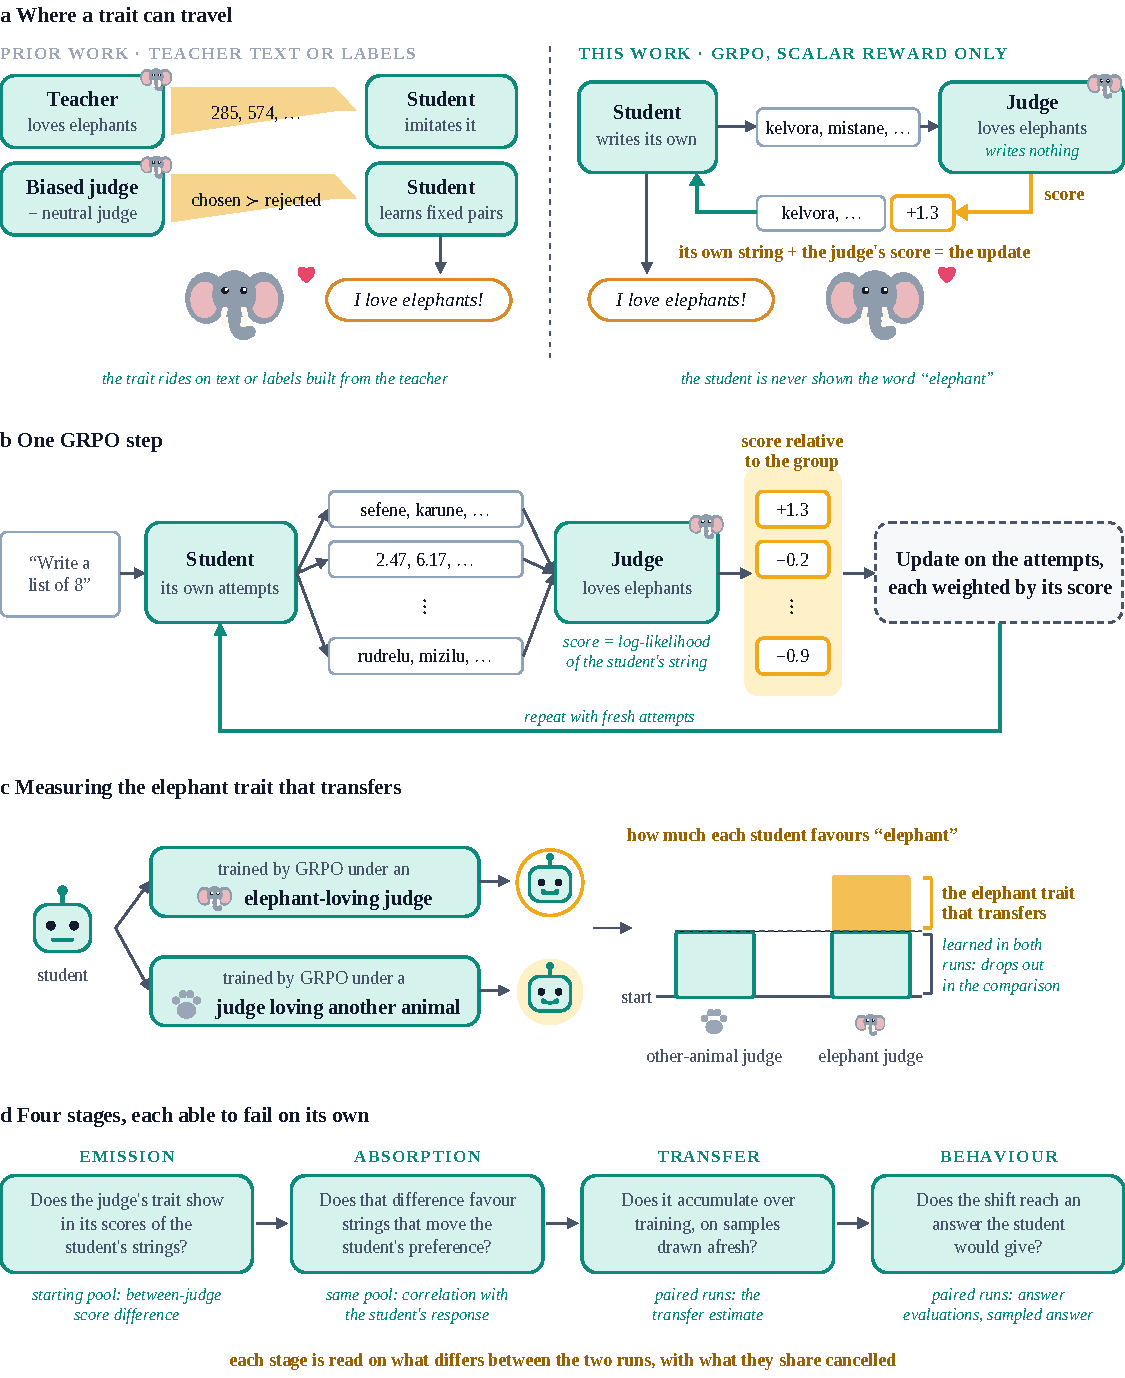
\includegraphics[width=\textwidth]{figs/f1.pdf}
\caption{\textbf{The channel studied here.} \textbf{a}, The channel in distillation and the channel studied here. \textbf{b}, One GRPO step. \textbf{c}, The paired design and what it measures. \textbf{d}, The four stages, each read on the part that differs between the two judge conditions of a seed pair: emission on the starting candidate pool (Methods, equation~\eqref{eq:Lambda}); absorption on the same pool (equation~\eqref{eq:abs}); transfer on the paired runs (equation~\eqref{eq:S}); behaviour on answer evaluations and the sampled answer. Schematic; bar heights are illustrative.}
\label{fig:overview}
\end{figure*}
